%\section{数据、信息与进位制}
\setcounter{section}{1}
\setcounter{subsection}{0}
\subsection{1.2 数据、信息与进位制}



\begin{compactenum}[1.]
%\labelwidth = 2em
\item \textbf{数据的定义}
	\begin{compactitem}
	\item 数据是对客观事物的符号表示。
	\item 在计算机科学中,数据表现形式可以是文字、图形、图像、音频、视频等。
	\end{compactitem}
\item \textbf{信息及信息的特征}
	\begin{compactitem}
	\item 信息是数据、信号中所包含的含义
	\item 信息具有\textbf{载体依附性}、时效性、共享性、可加工处理性等特征。
	\end{compactitem}
\item \textbf{知识}
	\begin{compactitem}
	\item 知识是人类在社会实践中所获得的认识和经验的总和,也是人类在实践中认识客观世界的成果,它包括对事实、信息的描述及在教育和实践中获得的技能。
	\item 知识是可以积累与传承的。
	\end{compactitem}
\item \textbf{数据、信息与知识的关系}
	\begin{compactitem}
	\item 数据经过解释后产生的意义就是信息,数据是信息的载体,单纯的数字是没有意义。
	\item 通过归纳、演绎、比较等手段对信息进行挖掘,将万千信息中有价值的部分与已存在的人类知识体系相结合,形成知识。
	\item 数据、信息与知识的关系可以通过图表示
	\end{compactitem}
\begin{figure}[!ht]
\centering
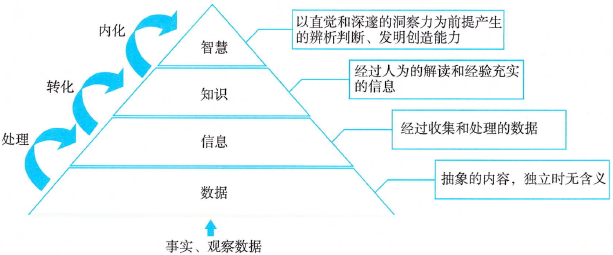
\includegraphics[width=0.5\linewidth]{pic/c01.01.info.knowledge}
\end{figure}


\item \textbf{数字化}
	\begin{compactitem}
	\item 将模拟信号转换为数字信号的过程称为数字化
	\item 将模拟信号转换成数字信号一般需要经过采样、量化与编码
	\end{compactitem}

\item \textbf{进制转换}
	\begin{compactitem}
	\item 将\underline{十进制$ \to k$进制}:\textbf{除$k$取余法},将\underline{$k$进制$\to$十进制}数可用\textbf{按权相加法}(即$\times \; k^{i-1}$),e.g.
		\begin{compactitem}[\ding{86}]
		\item $25D$=$11001B, \because $
		\[ \begin{aligned} 25 \div 2=12\cdots & {\color{red}1} \\
		12 \div 2=6\cdots & {\color{red}0} \\
		6 \div 2=3\cdots & {\color{red}0} \\
		3 \div 2=1\cdots & {\color{red}1} \\
		1 \div 2=0\cdots & {\color{red}1}
		\end{aligned} \]
		\item $D2H=208D, \because 13\times 16^1 + 2 \times 16^0=208$
		\end{compactitem}
	
	\item 二进制数转换成十六进制数,从二进制数的低位开始,每四位二进制数转换成一位十六进制数;反之,每一位十六进制数可转换成四位二进制数。e.g.
		\begin{compactitem}[\ding{86}]
		\item $D2H = 11010010B, \because \; D_{(16)} \to 13_{(10)} \to 1101_{(2)}, 2_{(16)} \to 2_{(10)} \to 11_{(2)}$
		\item $110111B = 37H, \because \; 0111_{(2)} \to 7_{(10)} \to 7_{(16)}, 11_{(2)} \to 3_{(10)} \to 3_{(16)}$
		\end{compactitem}
	\end{compactitem}

\end{compactenum}%


\begin{groups}


\group{单选题}{每题仅有一个正确选项}
\begin{questions}[rp]

%% =========== 1
\question
\smkai{(作业本1.1)}下列有关数据的说法,正确的是
\choice{数据必须由数字组成}
{虚假的数据不能承载任何信息}
{数据的价值往往取决于其所承载的信息}
{所有的数据都是人为创造的}
\begin{solution}
C。数据可以有多种表现形式,数字只是最常见的一种;虚假的数据也能承载信息;数据的价值主要体现在所承载的信息;并非所有的数据都是由人类创造的。
\end{solution}

%% =========== 2
\question
\smkai{(作业本1.1)}下列关于数据和信息的说法,正确的是
\choice{数据的表现形式只能是文字和图像}
{同一信息对所有人而言其价值是相同的}
{有数字才能被输入到计算机中进行处理}
{信息是数据经分析、解释后得到的}
\begin{solution}
D。数据的表现形式除了文字和图像,还可以是音频、视频等形式;同一信息对不同的人而言,其价值是不同的;能被计算机处理的数据可以是文字、图形、图像、音频、视频等形式;数据是信息的载体,经过对数据的分析﹑解释可以得到信息。
\end{solution}

%% =========== 3
\question
\smkai{(作业本1.1)}世界第一高峰──珠穆朗玛峰位于中国和尼泊尔两国边界上,海拔8848.86米,是喜马拉雅山脉的主峰。结合上述事例,下列关于数据、信息﹑知识的描述正确的是
\choice{若在纸上单独书写“8848.86”这个数,它就已经被赋予了一定的意义}
{当人们看到海拔8000多米的高度时,会联想到缺氧、寒冷等词汇,这是知识的体现}
{“珠穆朗玛峰峰顶海拔过高,不宜人类居住。”这体现了人类的智慧}
{不同国籍的人引用珠穆朗玛峰高度采用不同的数据,说明存在虚假数据}
\begin{solution}
B。单独的数字没有明确的含义,只有经过解释才具有意义,这个意义就是信息,所以选项A中的数还不是信息;选项B提及的高海拔地区缺氧、寒冷等情况,既是常识,也是知识;选项C中“不宜人类居住”这一结论,是根据已有的知识做出的判断,还没达到智慧的高度;珠穆朗玛峰的不同高度数据,是因采用标准不同造成的,不是虚假数据。所以本题选B。
\end{solution}

%% =========== 4
\question
\smkai{(作业本1.1)}下列关于数据和信息的说法,正确的是
\choice{数据自古就有,但信息只在计算机被发明后才出现}
{数据量的大小决定了其所承载信息价值的高低}
{同一数据出现在不同的应用情境,表示的信息可能不同}
{计算机技术的发展已经使人类可以处理世界上所有数据}
\begin{solution}
C。数据、信息自古就有;信息的价值是相对的,对于不同的人其价值可能不同,与数据量的大小并没有绝对的联系;同一数据出现在不同的语境或不同的应用情境中,有不同的含义;计算机可以提高数据处理的效率,但它不是万能的,不可能处理世界上所有的数据。
\end{solution}

%% =========== 5
\question
\smkai{(作业本1.1)}下列有关信息的说法,不正确的是
\choice{信息超出有效期后不再具有任何价值}
{信息无处不在,且呈现形式多样}
{信息的传播、存储必须依附于某种载体}
{信息经过加工、处理可以具有更高的使用价值}
\begin{solution}
A。超出有效期后的信息未必没有价值,如有时可以作为参考进行研究;B,C,D选项是信息的基本特征。
\end{solution}

%% =========== 6
\question
\smkai{(作业本1.1)}下列有关计算机处理数据的说法,不正确的是
\choice{用计算机处理数据可以获得较高的效率}
{数据量较大时,只有计算机才能进行处理}
{计算机已成为处理数据最主要的工具}
{计算机可以处理文字、图形、图像、音频、视频等数据}
\begin{solution}
B。计算机处理速度快,准确性高,所以处理数据效率高;数据量大用计算机处理效率高,但未必一定要用计算机处理,如在计算机出现之前人类也能处理大量数据,只是效率较低,用时较长;C、D选项是计算机特点与功能。
\end{solution}

%% =========== 7
\question
\smkai{(作业本1.1)}下列有关数据、信息和知识的说法,正确的是
\choice{一般而言,数据都是真实可信的,而信息可能存在虚假}
{人类能采集到的信息中都蕴含着很高的价值}
{只要有足够多的信息,就能建构任意知识}
{随着人类社会的发展,已有的知识也有可能继续完善}
\begin{solution}
D。数据也有可能存在虚假,一般由人为造成;并不是所有的信息都蕴含很高的价值;知识的建构并不是仅仅依靠简单的信息积累;在人类这社会发展过程中,知识也在不断传承与完善。
\end{solution}

%% =========== 8
\question
\smkai{(作业本1.1)}古代的数学家发现正多边形的边数越多,其形状就越接近于圆。魏晋时期数学家刘徽利用割圆术计算出圆周率的近似值为3.14,并以此来计算圆的面积。下列有关该事例中数据、信息、知识、智慧的说法,不正确的是
\choice{刘徽从正六边形开始,每次倍增边数,最后割成192边,该过程中采集到了数据}
{从此之后,3.14这个数据在任何地方都表示圆周率}
{刘徽采用割圆术这一方法,是智慧的体现}
{圆面积的近似值可以用3.14乘以半径的平方获得,这是知识}
\begin{solution}
B。割圆术方法中,正多边形的边数越多,则越接近圆,同时也为了记录圆周长;
只有在计算相关数据(如圆周长、面积等)时,3.14这个数字不用解释也有明确的意义;
对于创造性的思维方法属于智慧;
圆面积公式作为知识已经写入教材。
\end{solution}

%% =========== 9
\question
\smkai{(作业本1.2)}要表示$10$种不同的信息,需要的二进制位数至少为
\choice{1}
{2}
{4}
{10}
\begin{solution}
C。$n$位二进制数可以表示$2^n$种不同的信息,故答案为C。
\end{solution}

%% =========== 10
\question
\smkai{(作业本1.2)}有十进制数$115$,将其用一个字节的二进制表示,结果是
\choice{0111 0011}
{0011 0011}
{0110 0111}
{1100 1110}
\begin{solution}
A。可以用除二取余法得到,也可以根据127的二进制数是$1111111$B,再减去$12$(即$1100$)进行计算
\end{solution}

%% =========== 11
\question
\smkai{(作业本1.2)}十进制数$111$转换为十六进制是
\choice{$6F$}
{$D7$}
{$37$}
{$D3$}
\begin{solution}
A。可以用除十六取余法。
也可以先转换为二进制$1101111$,再转换为十六进制。
\end{solution}

%% =========== 12
\question
\smkai{(作业本1.2)}算式:$0110 1101B + 16D$的结果是
\choice{$1110 1101B$}
{$0111 1101B$}
{$80D$}
{$234D$}
\begin{solution}
B。十进制数16转换为二进制是$10000$,所以答案是B
\end{solution}

%% =========== 13
\question
\smkai{(作业本1.2)}某二进制数共$5$位,其中最低位和最高位均为$1$,其他位未知,该二进制数转换为十进制后的最小值和最大值分别是
\choice{9,15}
{17,31}
{33,63}
{32,64}
\begin{solution}
B。对于最低位和最高位均为1的二进制数,最小值为10001,最大值为11111,所以答案为B
\end{solution}

%% =========== 14
\question
\smkai{(作业本1.2)}某数学题如下:设$\{a_n\}$是集合$\{2^t+2^s | 0 \le s<t, s,t\in Z\}$中所有的数从小到大排列成的数列,即$a_1=3, a+2=5, a_3=6, a_4=9, a_5=10, a_6=12, \cdots$将数列$\{a_n\}$各项按照上小下大、左小右大的原则写成如下的三角形数表:
\begin{lstlisting}
      3
     5 6
   9 10 12
  *  *  *  *
*  *  *  *  *
\end{lstlisting}
那么,$a_{100}$是(提示,将前面几个数转成二进制找规律)
\choice{1}
{2}
{3}
{4}
\begin{solution}
A。第四行:17,18,20,24;第五行:33,34,36,40,48
将第三行数字转换为二进制,分别是1001,1010,1100,可以得出规律,每个数中有两个1,且最高位是1,另一个1从低位开始向高位移动。可以得出第四行的二进制数是:10001, 10010,10100,11000;
第五行的二进制数是:100001, 100010,100100,101000,110000。
再利用高斯公式或对算式$1+2+3+\cdots$直接相加,可知第14层最后一个数为第105项,第14层共有14个数,所以第100项是第14层的第9项,即$t=14,s=8$(从0开始,所以第9项$s$是8), $a_{100} = 2^{14}+2^8=16384+256= 16640$
\end{solution}

%% =========== 15
\question
\smkai{(作业本1.2)}在计算机中,原码和补码是两种常见的数字表示方法。\textbf{原码}表示法是在数值前面增加一位符号位(即最高位为符号位):正数为$0$,负数为$1$,其余位表示数值的大小。在\textbf{补码}表示法中,正整数的补码与原码相同,负整数的补码是将其原码除符号位外的所有位取反(0变1,1变0,符号位为1不变)后加1。若用一个字节来表示,则十进制数$-123$的\textbf{补码}是
\choice{11111011}
{01111011}
{10000100}
{10000101}
\begin{solution}
D。十进制数$123$用一个字节的二进制数表示是$01111011$,每位数字取反得到$10000100$,加$1$后得$10000101$
\end{solution}




\end{questions}
\end{groups}
